\documentclass[conference,10pt]{IEEEtran}
\usepackage[utf8]{inputenc}
\usepackage{amsmath,amssymb}
\usepackage{graphicx}
\usepackage{booktabs}
\usepackage{cite}
\usepackage{url}
\usepackage{multirow}
\usepackage{array}
\usepackage[hidelinks]{hyperref}
\usepackage{tikz}
\usetikzlibrary{shapes.geometric,arrows.meta,positioning,fit,calc}
\usepackage{balance}

\graphicspath{{figures/}}

\title{Optimal Co-location of Data Centers and Renewable Energy Systems in Caribbean Small Island Developing States: A PyPSA Framework with Multi-Criteria Siting Analysis}

\author{
\IEEEauthorblockN{Shankar Ramharack\IEEEauthorrefmark{1}, Patrick Hosein\IEEEauthorrefmark{2}, Sham Mahabir\IEEEauthorrefmark{1}, Rajiv Sahadeo\IEEEauthorrefmark{1}, Sanjay Bahadoorsingh\IEEEauthorrefmark{2}}
\IEEEauthorblockA{\IEEEauthorrefmark{1}IEEE Power \& Energy Society, Trinidad \& Tobago Section\\
\IEEEauthorrefmark{2}Department of Electrical \& Computer Engineering, The University of the West Indies, St.~Augustine\\
Email: shankar.ramharack@ieee.org}
}

\begin{document}
\maketitle

\begin{abstract}
The rapid expansion of data centers presents both economic opportunities and systemic risks for Caribbean Small Island Developing States~(SIDS). This paper develops a PyPSA-based capacity expansion framework for optimal co-location of data centers with renewable energy infrastructure, incorporating behind-the-meter battery storage, workload flexibility (70\%/30\% inflexible/flexible split), and multi-bus transmission topology. Two case studies are examined: Trinidad~\&~Tobago (single-bus, 92\,MW Brechin Castle solar, 5\,MW data center) and Jamaica (4-bus 138\,kV JPS network, 15\,MW data center at Kingston). Jamaica's optimum deploys 405\,MW solar, 278\,MW wind, 800\,MWh grid-scale BESS, and 84\,MWh behind-the-meter BESS, achieving 42.5\% renewable penetration. A post-hoc distributionally robust assessment evaluates hurricane resilience, and a novel 10-factor siting framework addresses the regulatory gap in SIDS that lack data-center-specific zoning. Results show that energy-optimal locations may score poorly on societal criteria---noise, freshwater stress, zoning readiness---demonstrating the need for integrated planning tools in small island contexts.
\end{abstract}

\begin{IEEEkeywords}
Data centers, renewable energy, capacity expansion, PyPSA, SIDS, Caribbean, behind-the-meter storage, workload flexibility, zoning, siting, resilience.
\end{IEEEkeywords}

% ══════════════════════════════════════════════════════
\section{Introduction}
% ══════════════════════════════════════════════════════

Global data center electricity consumption reached approximately 460\,TWh in 2024, with projections exceeding 1{,}000\,TWh by 2030 driven by artificial intelligence workloads~\cite{iea2024}. In the United States, over \$64~billion in data center projects have faced delays or cancellations from community opposition over noise, water consumption, and grid strain~\cite{dcwatch2025}. For Caribbean SIDS---small, import-dependent economies with fragile power grids and acute hurricane exposure---hosting data centers introduces systemic risks that existing planning frameworks do not address.

Jamaica's power system, operated by Jamaica Public Service Company~(JPS), serves approximately 650\,MW peak demand through 400\,km of 138\,kV and 800\,km of 69\,kV transmission connecting 52~substations~\cite{jps_grid}. A 15\,MW data center at Kingston would represent 2.3\% of peak demand. Trinidad~\&~Tobago's 1{,}800\,MW system---anchored by natural gas from the National Gas Company~(NGC) and recently augmented by the landmark 92\,MW Brechin Castle solar farm~\cite{brechin2025}---operates with substantial generation headroom, offering a contrasting context for co-planning analysis.

This paper contributes: (i)~a PyPSA-based co-planning framework with behind-the-meter~(BTM) storage, workload flexibility, and multi-bus transmission based on real JPS topology; (ii)~post-hoc distributionally robust hurricane resilience assessment; and (iii)~a 10-factor siting suitability framework for Caribbean SIDS.

% ══════════════════════════════════════════════════════
\section{Literature Review}
% ══════════════════════════════════════════════════════

\subsection{The Data Center Energy Problem}

Data centers are among the fastest-growing electricity consumers globally. The IEA estimates that AI-driven workloads alone could add 300--500\,TWh by 2030~\cite{iea2024}. Unlike traditional industrial loads, data centers exhibit unique characteristics that complicate grid integration: high power density (5--50\,MW per facility), near-perfect load factors (0.85--0.95), stringent reliability requirements (Tier~III/IV mandate 99.982\%+ uptime), and significant cooling loads that vary with ambient temperature. Google's 24/7 carbon-free energy~(CFE) initiative demonstrated that hourly matching of data center load to clean generation requires co-optimized storage and flexible scheduling~\cite{google247}. Microsoft's 2024 sustainability report identified workload flexibility as a key enabler, with 20--35\% of training and batch workloads being temporally shiftable~\cite{microsoft2024}.

The siting challenge has intensified. Power, water, and permitting have been identified as the three new pillars of site selection~\cite{dccom2025}. GE~Vernova's consulting framework evaluates grid congestion, climate resilience, and RE resource alignment~\cite{ge_vernova}. In the US, the ACM~COMPASS~2025 study documented that data center cooling systems generate 80--96\,dBA at source, and that Google consumed over 5~billion gallons of water globally in 2023~\cite{compass2025}. Jurisdictions have responded with increasingly specific regulations: 500-foot setbacks, mandatory acoustic modeling, and in some cases outright moratoria~\cite{stafford2025,albemarle2025}.

\subsection{Caribbean SIDS Energy Context}

Caribbean SIDS face electricity costs of \$0.25--0.45/kWh and heavy fossil dependence~\cite{ccreee2023}. Jamaica's RE penetration was 12\% in 2022~\cite{ccreee_jm}, with a government target of 50\% by 2030 supported by IRP-2~\cite{jm_irp2}. Trinidad~\&~Tobago is advancing its energy transition alongside its established gas sector; the Brechin Castle Solar Farm---a joint venture of bp, Shell, and NGC on 186~hectares near Couva---delivered first electrons in July~2025 and contributes approximately 8\% of total generation capacity when fully commissioned~\cite{brechin2025,brechin_bp}. This project demonstrates a replicable model of private-sector-led renewable deployment supported by government facilitation~\cite{brechin_ecp}. No Caribbean nation has data-center-specific zoning frameworks~\cite{uli2024}.

\subsection{Why PyPSA: Open-Source Capacity Expansion}

Energy system modeling tools range from commercial platforms (PLEXOS, HOMER Pro, Aurora) costing tens of thousands of dollars per license, to open-source frameworks. For SIDS---where government ministries, regulators, and academic institutions operate under severe budget constraints---licensing costs represent a material barrier. Table~\ref{tab:tools} compares frameworks relevant to this study.

\begin{table}[htbp]
\centering
\caption{Energy System Modeling Tools Comparison}
\label{tab:tools}
\setlength{\tabcolsep}{2.5pt}
\begin{tabular}{@{}lcccc@{}}
\toprule
Feature & PyPSA & GenX & PLEXOS & HOMER \\
\midrule
License & Free & Free & Comm. & Comm. \\
Language & Python & Julia & .NET & GUI \\
Multi-bus network & \checkmark & -- & \checkmark & -- \\
Sector coupling & \checkmark & \checkmark & \checkmark & Partial \\
Storage modeling & \checkmark & \checkmark & \checkmark & \checkmark \\
Open solver (HiGHS) & \checkmark & \checkmark & -- & -- \\
Active community & \checkmark & \checkmark & -- & -- \\
PyPSA-Earth (global) & \checkmark & -- & -- & -- \\
\bottomrule
\end{tabular}
\end{table}

PyPSA~\cite{pypsa} was selected for its combination of: (i)~free, open-source licensing under MIT terms; (ii)~native multi-bus network modeling with transmission constraints; (iii)~compatibility with the open-source HiGHS solver, eliminating dependence on commercial solvers like Gurobi or CPLEX~\cite{highs}; (iv)~an active development community and the PyPSA-Earth project providing global coverage~\cite{pypsa_earth}; and (v)~a Python-based API accessible to researchers and practitioners in SIDS without specialized commercial software training. PyPSA's graph-based architecture scales naturally from single-bus to continental networks, making it suitable for both the Trinidad single-bus and Jamaica 4-bus cases examined here.

% ══════════════════════════════════════════════════════
\section{Methodology}
% ══════════════════════════════════════════════════════

Fig.~\ref{fig:workflow} presents the integrated methodology.

\begin{figure}[htbp]
\centering
\resizebox{\columnwidth}{!}{%
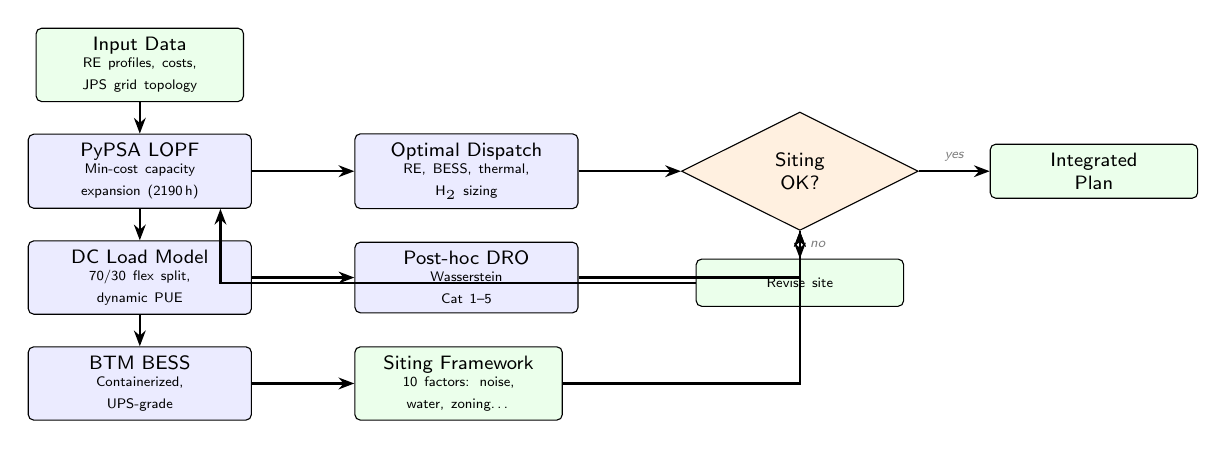
\begin{tikzpicture}[
  block/.style={rectangle, draw, fill=blue!8, text width=2.6cm, minimum height=0.7cm, align=center, font=\scriptsize\sffamily, rounded corners=2pt},
  decision/.style={diamond, draw, fill=orange!12, text width=1.4cm, minimum height=0.6cm, align=center, font=\scriptsize\sffamily, aspect=2},
  io/.style={rectangle, draw, fill=green!8, text width=2.4cm, minimum height=0.6cm, align=center, font=\scriptsize\sffamily, rounded corners=2pt},
  arr/.style={-{Stealth[length=2mm]}, thick},
  lab/.style={font=\tiny\sffamily\itshape, text=gray}
]
\node[io] (inp) {Input Data\\{\tiny RE profiles, costs,\\JPS grid topology}};
\node[block, below=0.4cm of inp] (pypsa) {PyPSA LOPF\\{\tiny Min-cost capacity\\expansion (2190\,h)}};
\node[block, below=0.4cm of pypsa] (dc) {DC Load Model\\{\tiny 70/30 flex split,\\dynamic PUE}};
\node[block, below=0.4cm of dc] (btm) {BTM BESS\\{\tiny Containerized,\\UPS-grade}};
\node[block, right=1.3cm of pypsa] (opt) {Optimal Dispatch\\{\tiny RE, BESS, thermal,\\H$_2$ sizing}};
\node[block, right=1.3cm of dc] (dro) {Post-hoc DRO\\{\tiny Wasserstein\\Cat 1--5}};
\node[io, right=1.3cm of btm] (site) {Siting Framework\\{\tiny 10 factors: noise,\\water, zoning\ldots}};
\node[decision, right=1.3cm of opt] (integ) {Siting\\OK?};
\node[io, right=0.9cm of integ] (out) {Integrated\\Plan};
\node[io, below=0.35cm of integ] (rev) {\tiny Revise site};
\draw[arr] (inp) -- (pypsa); \draw[arr] (pypsa) -- (dc); \draw[arr] (dc) -- (btm);
\draw[arr] (pypsa) -- (opt); \draw[arr] (dc) -- (dro); \draw[arr] (btm) -- (site);
\draw[arr] (opt) -- (integ); \draw[arr] (dro) -| (integ); \draw[arr] (site) -| (integ);
\draw[arr] (integ) -- node[above,lab]{yes} (out);
\draw[arr] (integ) -- node[right,lab]{no} (rev);
\draw[arr] (rev) -| ([xshift=-0.4cm]pypsa.south east);
\end{tikzpicture}
}
\caption{Integrated methodology: PyPSA capacity expansion combined with post-hoc resilience assessment and multi-criteria siting evaluation.}
\label{fig:workflow}
\end{figure}

\subsection{Capacity Expansion Formulation}

The framework minimizes total annualized system cost over snapshots $\mathcal{T}$ ($|\mathcal{T}| = 2{,}190$\,h). Capital costs are scaled by $\alpha = |\mathcal{T}|/8760$ to maintain correct annualized economics for sub-annual simulation:
\begin{equation}
\min_{\substack{p_{g,t},\, \bar{G}_g \\ e_{s,t},\, \bar{E}_s}} \;\sum_{g \in \mathcal{G}} \left(\alpha\, c_g^{\text{inv}} \bar{G}_g + \sum_{t} c_g^{\text{mc}} p_{g,t}\right) + \sum_{s \in \mathcal{S}} \alpha\, c_s^{\text{inv}} \bar{E}_s
\label{eq:obj}
\end{equation}
where annualized investment cost uses the capital recovery factor:
\begin{equation}
c_g^{\text{inv}} = \text{CAPEX}_g \cdot \frac{r(1+r)^{n_g}}{(1+r)^{n_g}-1} + \text{OPEX}_g
\label{eq:crf}
\end{equation}
with weighted average cost of capital $r$ and asset lifetime $n_g$.

\noindent\textbf{Nodal power balance} at each bus~$b$ and snapshot~$t$:
\begin{equation}
\sum_{g \in \mathcal{G}_b} p_{g,t} + \sum_{l \in \mathcal{L}_b^{+}} \eta_l f_{l,t} - \sum_{l \in \mathcal{L}_b^{-}} f_{l,t} = d_{b,t}^{\text{grid}} + d_{b,t}^{\text{DC}} \quad \forall\, b,t
\label{eq:balance}
\end{equation}
where $f_{l,t}$ is the power flow on link~$l$ and $\eta_l$ is its efficiency (capturing ohmic losses on the 138\,kV backbone: $\eta_{\text{KGN-OH}}=0.990$, $\eta_{\text{OH-MP}}=0.985$, $\eta_{\text{MP-MB}}=0.975$).

\noindent\textbf{Generator bounds} enforce minimum stable generation and time-varying capacity factors for variable RE:
\begin{equation}
\underline{p}_g (\bar{G}_g^{0} + \bar{G}_g) \leq p_{g,t} \leq \bar{p}_{g,t}\, (\bar{G}_g^{0} + \bar{G}_g) \quad \forall\, g,t
\label{eq:gen}
\end{equation}
where $\bar{G}_g^{0}$ is existing (fixed) capacity, $\bar{G}_g$ is optimized new capacity, $\underline{p}_g$ is the minimum stable output fraction (e.g., 0.40 for JEP LNG, 0.35 for HFO), and $\bar{p}_{g,t} \in [0,1]$ is the capacity factor profile for solar and wind generators.

\noindent\textbf{Transmission flow bounds}:
\begin{equation}
0 \leq f_{l,t} \leq \bar{F}_l \quad \forall\, l,t
\label{eq:tx}
\end{equation}
where $\bar{F}_l$ is the thermal rating (300/200/180\,MW for the three Jamaica corridors).

\noindent\textbf{Store energy balance} with cyclic boundary condition:
\begin{equation}
e_{s,t} = e_{s,t-1} + \eta_s^{+} p_{s,t}^{+} - \frac{p_{s,t}^{-}}{\eta_s^{-}}, \quad e_{s,0} = e_{s,|\mathcal{T}|}
\label{eq:store}
\end{equation}
where $\eta_s^{+}$, $\eta_s^{-}$ are charge/discharge efficiencies. Grid-scale BESS uses $\eta_{\text{RT}} = 0.865$ (round-trip); BTM BESS uses $\eta_{\text{RT}} = 0.846$ reflecting tropical derate and containerized power electronics.

\subsection{Data Center Load Model}

DC electrical demand decomposes into inflexible (latency-sensitive) and flexible (batch/training) components:
\begin{equation}
d_t^{\text{DC}} = \underbrace{(1-\phi)\, P_t^{\text{IT}}\, \text{PUE}(T_t)}_{\text{inflexible}} + \underbrace{\phi\, \overline{P^{\text{IT}} \cdot \text{PUE}}^{\,\text{day}}}_{\text{flexible (daily avg.)}}
\label{eq:dc}
\end{equation}
with flexible fraction $\phi=0.30$ and dynamic PUE responding to ambient temperature:
\begin{equation}
\text{PUE}(T_t) = \text{PUE}_{\text{nom}}\bigl(1 + 0.005\,(T_t - 25\,^\circ\text{C})\bigr)
\label{eq:pue}
\end{equation}
The IT load $P_t^{\text{IT}}$ exhibits diurnal variation ($\pm 6\%$, peak at 14:00) and weekday/weekend modulation (12\% reduction on weekends). The flexible portion is modeled as a daily-averaged flat load, representing the optimizer's freedom to shift batch workloads within a 24-hour window without introducing additional integer or store-based decision variables.

\subsection{Behind-the-Meter BESS}

BTM storage is modeled as a dedicated store connected exclusively to the DC bus, separate from grid-scale BESS. The BTM carries a 19\% cost premium over grid-scale (\$250 vs.\ \$210/kWh) reflecting containerized UPS-grade packaging and shorter warranty life (12 vs.\ 15 years). The charge/discharge links use $\eta=0.92$ per direction (vs.\ 0.93 for grid-scale). BTM and grid BESS are co-optimized within the same LP, allowing the solver to determine whether local or centralized storage is more economical at each bus.

\subsection{Post-Hoc DRO Resilience}

Hurricane resilience is assessed outside the main optimization using a distributionally robust framework. For each island~$i$, we define categorical damage profiles $\{(p_c, g_c, h_c)\}_{c=1}^{5}$ where $p_c$ is the empirical probability of category~$c$, $g_c$ is the fractional grid outage, and $h_c$ is the outage duration (hours). The worst-case expected unserved energy under a Wasserstein ambiguity set of radius $\varepsilon$ is:
\begin{equation}
R_i(\varepsilon) = 1 - \frac{\sup_{\mathbb{Q} \in \mathcal{B}_\varepsilon(\hat{\mathbb{P}})} \mathbb{E}_\mathbb{Q}[\text{UE}_i]}{P_i^{\text{DC}} \cdot 8760}
\label{eq:dro}
\end{equation}
where the Wasserstein ball $\mathcal{B}_\varepsilon(\hat{\mathbb{P}}) = \{\mathbb{Q} : W_1(\mathbb{Q}, \hat{\mathbb{P}}) \leq \varepsilon\}$ captures distributional uncertainty in hurricane frequency under climate change scenarios. The island-specific strike probability $s_i$ modulates the base category distribution (e.g., $s_{\text{Trinidad}} = 0.3$, $s_{\text{Jamaica}} = 0.8$). BESS provides partial backup proportional to $(1 - 0.3 \cdot g_c)$, capturing reduced but non-zero storage availability during storms.

% ══════════════════════════════════════════════════════
\section{Case Studies}
% ══════════════════════════════════════════════════════

\subsection{Case A: Trinidad \& Tobago (Fig.~\ref{fig:trinidad})}

Single-bus: 1{,}800\,MW gas fleet, Brechin Castle 92\,MWac solar~(bp/Shell/NGC joint venture, commissioned 2025, the Caribbean's largest utility-scale PV~\cite{brechin2025}), extendable solar (300\,MW), wind (100\,MW), grid BESS (400\,MWh), H$_2$ (20\,MW). WACC~7\%. DC: 5\,MW~IT at Point Lisas Industrial Estate, PUE~1.5, 30\%~flexible, 30\,MWh BTM.

Trinidad~\&~Tobago's energy landscape is evolving: while natural gas remains the backbone of electricity generation, the Brechin Castle project signals a strategic diversification pathway. The model captures both the existing gas fleet and the new solar capacity, reflecting the nation's current energy mix without prejudging future policy directions.

\begin{figure}[htbp]
\centering
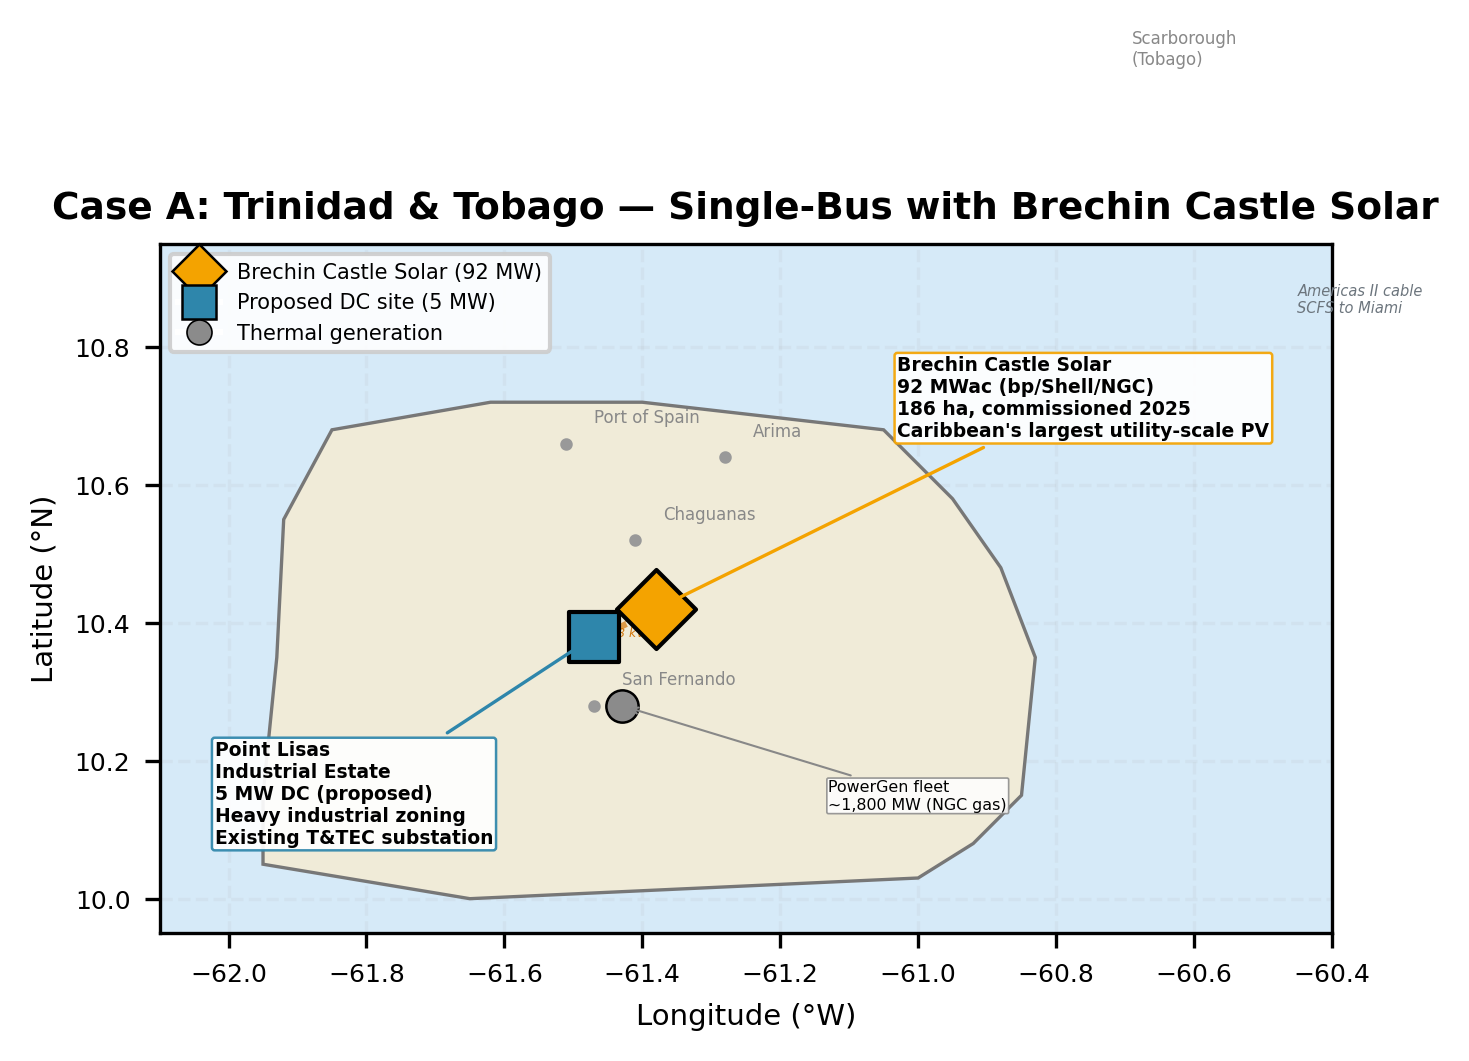
\includegraphics[width=\columnwidth]{fig1b_trinidad.png}
\caption{Case A: Trinidad \& Tobago. Brechin Castle Solar (92\,MWac) and proposed 5\,MW data center at Point Lisas Industrial Estate.}
\label{fig:trinidad}
\end{figure}

\subsection{Case B: Jamaica (Fig.~\ref{fig:jamaica})}

Four buses model the JPS 138\,kV backbone: \textbf{Kingston}~(load centre, Hunts Bay 150\,MW, JPPC/Rockfort 120\,MW diesel, Content Solar 37\,MW, \emph{15\,MW DC}); \textbf{Old Harbour}~(JEP 190\,MW LNG combined-cycle~\cite{jep2019}, 120\,MW legacy HFO, brownfield solar 150\,MW); \textbf{May Pen}~(Wigton Wind 100\,MW~\cite{wigton}, 29\,MW hydro, Eight Rivers Solar 20\,MW, extendable solar 400\,MW); \textbf{Montego Bay}~(Bogue 120\,MW GT, extendable wind 300\,MW). Transmission: KGN--OH 300\,MW (20\,km, recently upgraded~\cite{jps_upgrade}), OH--MP 200\,MW (40\,km), MP--MB 180\,MW (100\,km). WACC~10\%.

\begin{table}[htbp]
\centering
\caption{Technology Cost Assumptions (IRENA 2023~\cite{irena2023}, Caribbean premiums applied)}
\label{tab:costs}
\setlength{\tabcolsep}{3pt}
\begin{tabular}{@{}lcccc@{}}
\toprule
Technology & CAPEX & OPEX & Life & Source \\
\midrule
Solar PV & \$1{,}100/kW & \$12/kW/yr & 25\,yr & \cite{irena2023} \\
Onshore wind & \$1{,}600/kW & \$35/kW/yr & 20\,yr & \cite{irena2023} \\
Grid BESS (4h) & \$210/kWh & \$4/kWh/yr & 15\,yr & \cite{irena2023} \\
BTM BESS (4h) & \$250/kWh & \$5/kWh/yr & 12\,yr & Est.\ (+19\%) \\
PEM electrolyzer & \$1{,}400/kW & \$28/kW/yr & 20\,yr & \cite{irena2023} \\
\bottomrule
\end{tabular}
\end{table}

\noindent All profiles use synthetic AR(1)-modulated solar/wind capacity factors calibrated to Caribbean averages (solar CF\,0.18--0.21, wind CF\,0.22--0.30). The simulation covers Q1 (2{,}190\,h) with investment costs scaled by $\alpha = 2190/8760$.

\begin{figure}[htbp]
\centering
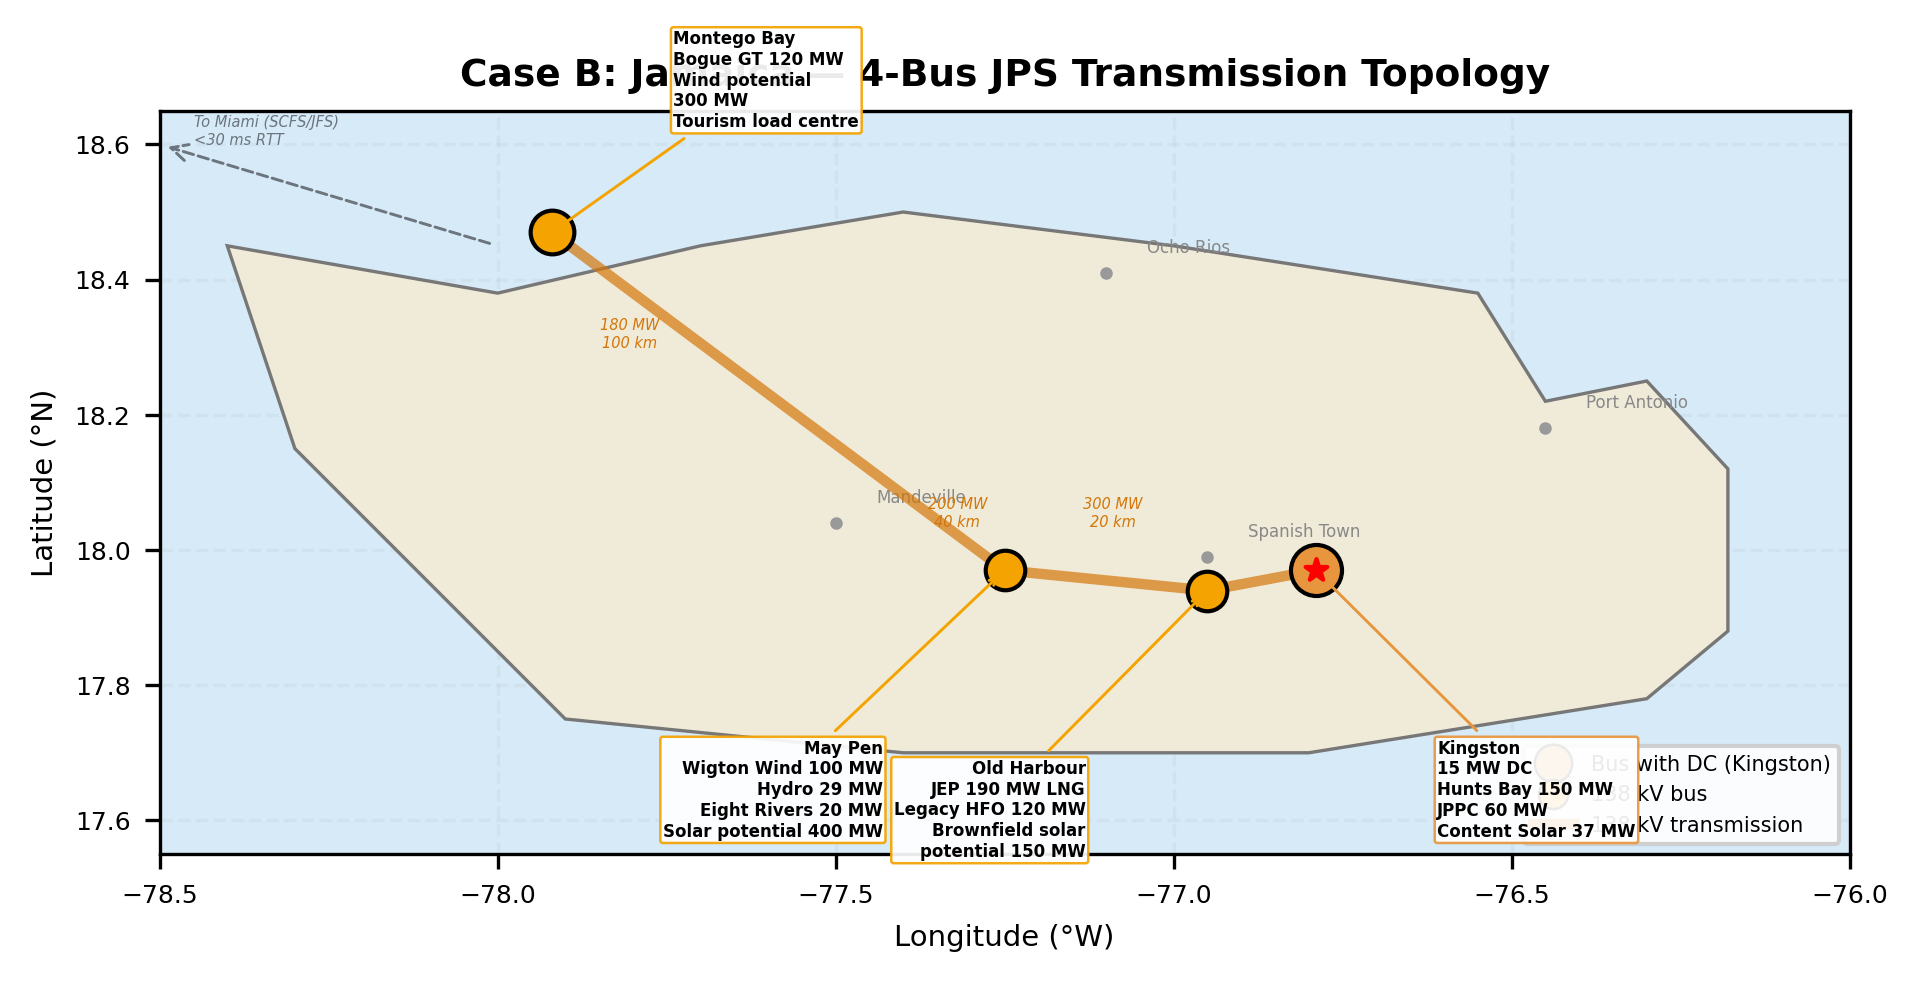
\includegraphics[width=\columnwidth]{fig1a_jamaica.png}
\caption{Case B: Jamaica 4-bus topology based on JPS 138\,kV backbone. Buses correspond to real substations. Red star marks the 15\,MW DC at Kingston.}
\label{fig:jamaica}
\end{figure}

% ══════════════════════════════════════════════════════
\section{Results}
% ══════════════════════════════════════════════════════

Table~\ref{tab:results} and Fig.~\ref{fig:results} summarize the optimized outcomes.

\begin{table}[htbp]
\centering
\caption{Optimization Results (Annualized)}
\label{tab:results}
\begin{tabular}{@{}lcc@{}}
\toprule
Metric & Case A: Trinidad & Case B: Jamaica \\
\midrule
System cost (M\,USD/yr) & 443 & 511 \\
RE fraction (\%) & 1.8 & 42.5 \\
New solar (MW) & 0 & 405 \\
New wind (MW) & 0 & 278 \\
Grid BESS (MWh) & 0 & 800 \\
BTM BESS (MWh) & 0 & 84 \\
CO$_2$ (kt/yr) & 2{,}983 & 1{,}198 \\
\bottomrule
\end{tabular}
\end{table}

\begin{figure}[htbp]
\centering
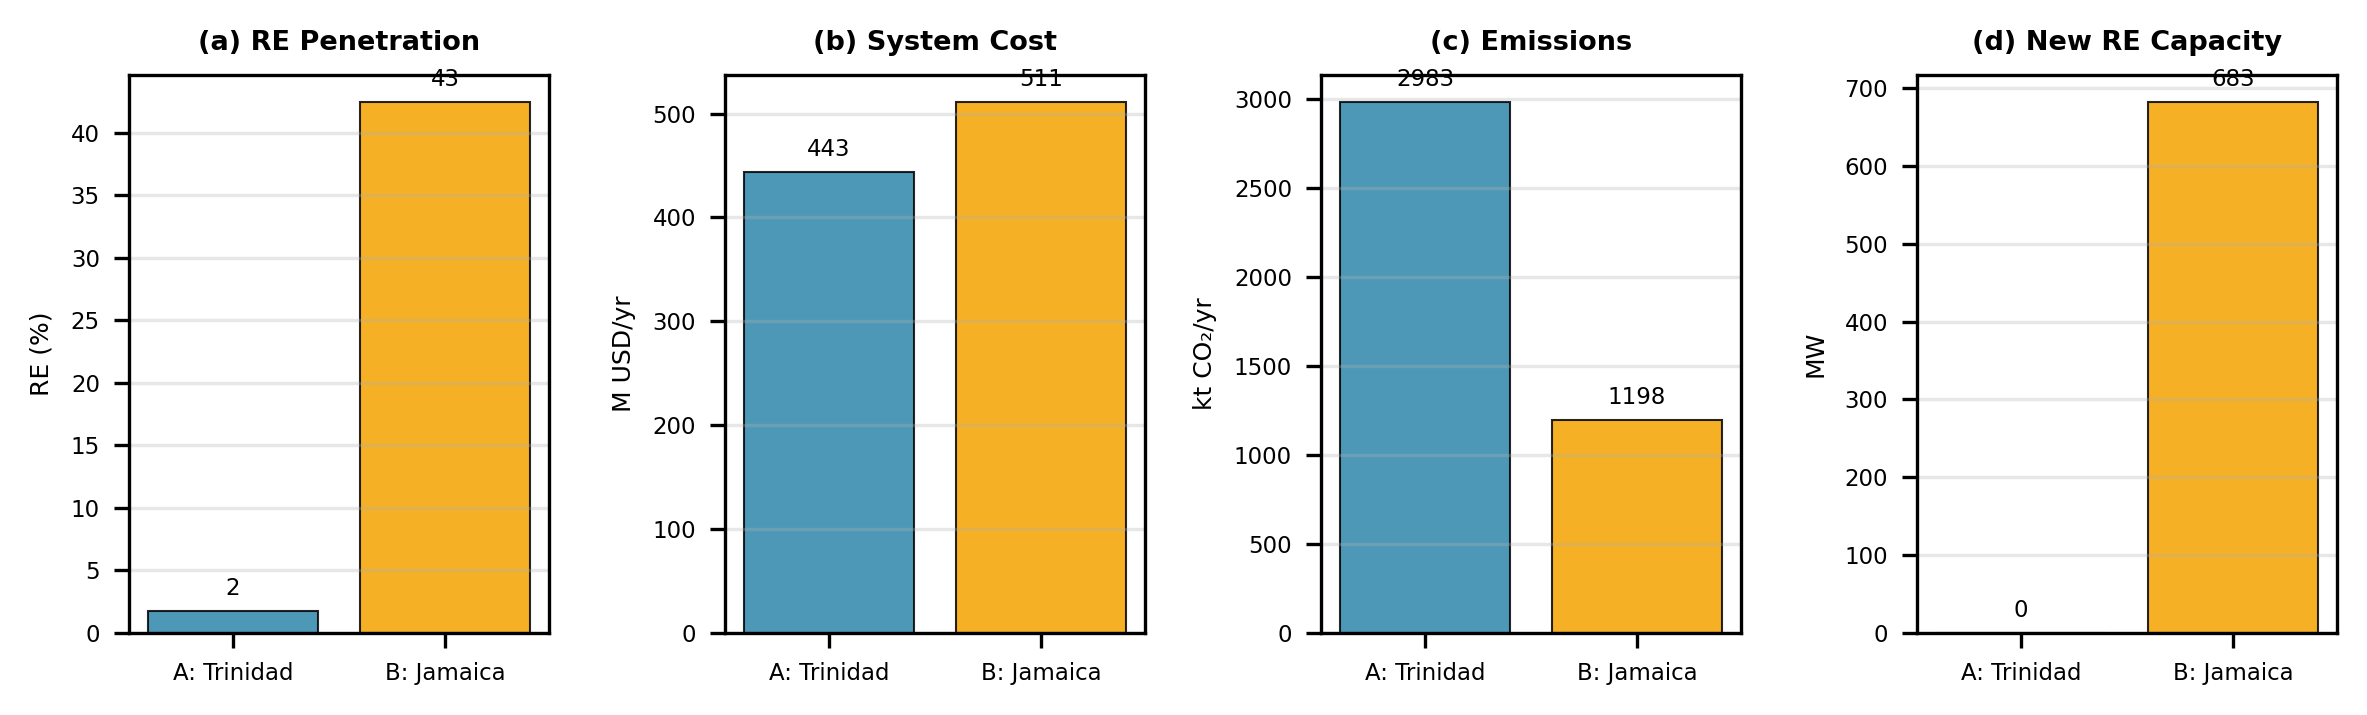
\includegraphics[width=\columnwidth]{fig2_results.png}
\caption{Optimization results: (a)~RE penetration, (b)~annualized system cost, (c)~CO$_2$ emissions, (d)~total new RE capacity.}
\label{fig:results}
\end{figure}

\textbf{Trinidad}: The optimizer deploys Brechin Castle's 92\,MW solar output (1.8\% RE fraction) but builds no additional RE or storage. The existing gas fleet serves the 5\,MW DC and national demand at competitive marginal cost. This outcome reflects the current economic reality of Trinidad's energy system, where abundant domestic gas provides reliable, low-cost baseload. Importantly, however, the framework could be applied to scenario analyses exploring future conditions---such as evolving gas allocation strategies or expanded RE targets---where additional solar and storage investment may become economically attractive.

\textbf{Jamaica}: The optimizer aggressively deploys 405\,MW solar (maxing May Pen and Old Harbour caps) and 278\,MW wind at Montego Bay, with 800\,MWh grid BESS at Kingston and Old Harbour. Notably, 84\,MWh BTM BESS deploys at the Kingston DC bus. BTM deployment is driven by transmission congestion: during peak coincident DC and grid demand, the KGN--OH corridor (300\,MW) constrains RE imports from central parishes, making local storage at the DC bus economically justified. Jamaica's 42.5\% RE aligns with its government's 50\% by 2030 target.

\textbf{DRO Resilience}: Trinidad maintains $R > 0.988$ across all Wasserstein radii due to its position south of the main hurricane belt (10.5$^\circ$N) and diverse generation. Jamaica degrades from $R = 0.995$ to $R = 0.970$ at $\varepsilon = 0.20$, driven by wind asset vulnerability. The 84\,MWh BTM provides approximately 4~hours of islanded DC backup.

% ══════════════════════════════════════════════════════
\section{Multi-Criteria Siting Framework}
% ══════════════════════════════════════════════════════

PyPSA determines \emph{where to build generation}; it does not assess whether a data center is \emph{socially and regulatorily feasible} at a given site. Caribbean SIDS lack the zoning frameworks that US jurisdictions have adopted in response to community opposition~\cite{dcwatch2025,stafford2025,albemarle2025,ramboll2024}. We propose a 10-factor framework calibrated to Caribbean conditions (Table~\ref{tab:siting}).

\begin{table}[htbp]
\centering
\caption{DC Siting Suitability Framework (1--5 scale, 5\,=\,best)}
\label{tab:siting}
\setlength{\tabcolsep}{2.5pt}
\begin{tabular}{@{}p{3.0cm}ccccc@{}}
\toprule
Factor & TT & JM-KGN & JM-OH & JM-MB \\
\midrule
\multicolumn{5}{@{}l}{\textit{Energy \& Infrastructure}} \\
\;\; Grid headroom & 5 & 3 & 4 & 2 \\
\;\; RE resource quality & 3 & 3 & 4 & 5 \\
\;\; Transmission adequacy & 5 & 4 & 4 & 2 \\
\multicolumn{5}{@{}l}{\textit{Connectivity}} \\
\;\; Submarine fibre RTT & 4 & 5 & 3 & 3 \\
\;\; IX/peering proximity & 3 & 4 & 1 & 2 \\
\multicolumn{5}{@{}l}{\textit{Environmental \& Climate}} \\
\;\; Hurricane exposure & 5 & 3 & 3 & 2 \\
\;\; Water availability & 4 & 3 & 4 & 3 \\
\;\; Seismic risk & 4 & 3 & 3 & 3 \\
\multicolumn{5}{@{}l}{\textit{Societal \& Regulatory}} \\
\;\; Noise buffer feasibility & 4 & 2 & 4 & 3 \\
\;\; Zoning readiness & 4 & 3 & 3 & 2 \\
\midrule
\textbf{Total (unweighted)} & \textbf{41} & \textbf{33} & \textbf{33} & \textbf{27} \\
\bottomrule
\end{tabular}
\end{table}

\textbf{Key finding}: Old Harbour---not Kingston---emerges as Jamaica's strongest DC site (tied at 33, but with superior noise/water/grid attributes). This is a brownfield industrial location near the JEP LNG plant with existing 138\,kV connectivity. The energy optimization placed the DC at Kingston for latency; the siting framework reveals Old Harbour may be more feasible, illustrating the tension this framework is designed to surface.

% ══════════════════════════════════════════════════════
\section{Critical Assessment}
% ══════════════════════════════════════════════════════

We identify five categories of weakness in this work and suggest paths for future improvement.

\textit{1) Synthetic profiles}: All RE capacity factors and load profiles are generated from AR(1) stochastic models calibrated to Caribbean averages rather than measured meteorological or SCADA data. This introduces unquantified bias in temporal correlations. Future work should incorporate ERA5 reanalysis data or locally measured irradiance/wind speed time series.

\textit{2) Sub-annual simulation}: The Q1 snapshot (2{,}190\,h) captures dry-season trade-wind patterns but underrepresents hurricane season (Aug--Nov) and wet-season hydro variability. The scaling factor $\alpha = 2190/8760$ assumes Q1 is representative of annualized economics, which may overvalue dry-season wind and undervalue storage needed for hurricane resilience. Full 8{,}760-hour simulation---or representative period selection via k-medoids clustering---would improve robustness.

\textit{3) Simplified workload flexibility}: The daily-average flattening model understates the value of hourly temporal shifting. A full formulation using store-based shift operators~\cite{google247} or explicit bin-packing constraints would better capture RE--DC synergies, at the cost of significantly increased LP complexity.

\textit{4) Missing economic dimensions}: The LP captures energy arbitrage but not demand charges, capacity markets, or ancillary service revenues that drive BTM deployment in practice. No carbon price or emission constraint is modeled. Sector coupling (waste heat recovery via absorption chillers, COP~$\approx$\,0.7) could offset 15--20\% of cooling electricity but adds multi-carrier complexity.

\textit{5) Siting score subjectivity}: The 10-factor framework uses expert-assigned scores rather than quantitative indices with defined rubrics. Weighting is uniform, yet factors like submarine cable latency may dominate for certain workload profiles. A formal multi-criteria decision analysis (MCDA) with stakeholder-elicited weights~\cite{uli2024} and sensitivity analysis over weight vectors would strengthen the framework's policy relevance.

\textit{6) Network simplification}: The 4-bus Jamaica model captures major transmission corridors but omits the 69\,kV sub-transmission network, reactive power constraints, and N-1 contingency analysis required by the JPS Transmission Code~\cite{jps_grid}. More detailed representations using PyPSA-Earth workflows could address this gap.

% ══════════════════════════════════════════════════════
\section{Discussion}
% ══════════════════════════════════════════════════════

\textit{Why this work matters for Caribbean SIDS}: No published study applies open-source capacity expansion modeling to data center co-planning in the Caribbean. The combination of PyPSA optimization with a societal siting framework addresses a gap where existing tools focus exclusively on either energy economics (HOMER, PLEXOS) or real estate considerations (CBRE, JLL reports), but never both. For SIDS policymakers evaluating data center proposals---which increasingly arrive as unsolicited foreign direct investment---the framework provides a transparent, reproducible, and license-free assessment methodology that does not require commercial software procurement or external consulting fees.

\textit{Transmission reveals what single-bus hides}: Jamaica's 4-bus model shows RE concentrating at May Pen (solar) and Montego Bay (wind) while DC demand sits at Kingston. The MP--MB corridor (180\,MW, 100\,km through mountainous terrain) is the binding constraint, explaining why 800\,MWh of grid BESS deploys at Kingston and Old Harbour rather than at RE-rich buses. In a single-bus (copper-plate) model, this congestion is invisible, BTM BESS never deploys, and the total system cost is underestimated. This finding has direct implications for Jamaica's IRP-2 process, which uses simplified single-bus models for some analyses.

\textit{The Brechin Castle model for SIDS}: Trinidad's Brechin Castle project---a bp/Shell/NGC joint venture delivering 92\,MWac on 186~hectares---demonstrates a replicable model for Caribbean RE deployment. The consortium structure, with international energy companies partnering a national gas company and government facilitation without direct equity, addresses the financing and technical capacity constraints that impede utility-scale RE in smaller SIDS~\cite{brechin_ecp}. A data center co-located at Point Lisas could leverage both the existing industrial zoning and the adjacent solar generation, reducing the need for long-distance transmission.

\textit{Societal factors dominate SIDS siting}: On small islands, a 500-foot setback requirement---now standard in Virginia~\cite{stafford2025}---may consume a significant fraction of available industrial land. In Dominica or St.~Kitts, such a buffer could extend across the entire width of a coastal settlement. Even in Jamaica (10{,}990\,km$^2$), industrial zones are concentrated in a few corridors. The Point Lisas Industrial Estate in Trinidad and Old Harbour in Jamaica offer rare exceptions where heavy industrial zoning with adequate buffer zones already exists. Future Caribbean DC development should prioritize such brownfield sites rather than greenfield development that would require new zoning frameworks.

\textit{Water as a binding constraint}: A 15\,MW data center using evaporative cooling consumes approximately 50\,ML/yr~\cite{compass2025}. On water-stressed islands, this is not merely an operational concern but a potential trigger for community opposition, as documented in US contexts where data centers have been accused of depleting municipal water supplies~\cite{dcwatch2025}. Closed-loop or air-cooled alternatives add 15--25\% to cooling CAPEX but may be mandatory for SIDS. This cost premium is not captured in the current optimization and should be incorporated in future work.

\textit{Policy recommendations}: Caribbean SIDS should (i)~develop data-center-specific zoning addressing noise (45--55\,dBA limits), water usage caps, and setback distances scaled to island geography; (ii)~require co-located RE and BTM storage as permit conditions; and (iii)~prioritize brownfield industrial sites where infrastructure and buffer zones exist.

% ══════════════════════════════════════════════════════
\section{Conclusion}
% ══════════════════════════════════════════════════════

This paper presented a PyPSA framework for DC--RE co-planning in Caribbean SIDS. Jamaica's 4-bus model, grounded in real JPS topology, deploys 84\,MWh BTM BESS at the DC bus due to transmission congestion---a result invisible in single-bus analysis. The 10-factor siting framework reveals that Old Harbour, not Kingston, may be Jamaica's most suitable DC location when societal factors are considered. For Trinidad, the Brechin Castle solar project---a consortium of bp, Shell, and NGC delivering 92\,MWac adjacent to the Point Lisas industrial corridor---demonstrates a replicable pathway for RE integration that future DC developments could directly leverage.

The key message is that energy optimization alone is insufficient: societal impact, regulatory readiness, and climate resilience must be co-evaluated. As data center demand reaches Caribbean shores, integrated tools combining open-source capacity optimization with multi-criteria siting assessment will be essential for ensuring these developments serve the interests of small island communities.

\textbf{Future work} should pursue four directions: (i)~full 8{,}760-hour simulation with ERA5 reanalysis-derived profiles to eliminate seasonal bias; (ii)~formal MCDA with stakeholder-elicited weights for the siting framework; (iii)~extension to additional SIDS contexts (Barbados, Eastern Caribbean states, Pacific SIDS) where grid characteristics differ; and (iv)~incorporation of carbon pricing and NDC emission constraints into the PyPSA formulation to capture the full policy landscape of Caribbean energy transition.

\section*{Acknowledgments}

The authors gratefully acknowledge the developers of PyPSA~\cite{pypsa} and the HiGHS solver team~\cite{highs} for providing free, open-source tools that make energy system modeling accessible to SIDS researchers. We thank IRENA~\cite{irena2023}, the IEA~\cite{iea2024}, and CCREEE~\cite{ccreee2023} for publicly available cost benchmarks and Caribbean energy data. The JPS Book of Codes~\cite{jps_grid} and the Data Center Watch project~\cite{dcwatch2025} provided essential infrastructure and siting data respectively. The Brechin Castle Solar project documentation~\cite{brechin2025,brechin_bp} informed the Trinidad case study parameters.

\balance

\begin{thebibliography}{00}

\bibitem{iea2024} International Energy Agency, ``Electricity 2024: Analysis and forecast to 2026,'' IEA, Paris, 2024.

\bibitem{dcwatch2025} Data Center Watch, ``\$64 billion of data center projects blocked or delayed,'' Mar.~2025.

\bibitem{jps_grid} Jamaica Public Service Co., ``Jamaica Electricity Sector Book of Codes,'' Office of Utilities Regulation, Kingston, 2016.

\bibitem{brechin2025} Energy Chamber of Trinidad and Tobago, ``Brechin Castle Solar Farm set to launch in 2025,'' May~2025.

\bibitem{brechin_bp} bp Trinidad and Tobago, ``Brechin Castle Solar Limited achieves first electrons,'' Jul.~2025.

\bibitem{brechin_ecp} Energy Capital \& Power, ``How Trinidad's 92\,MW Brechin Castle project tests the Caribbean's clean energy ambitions,'' Dec.~2025.

\bibitem{google247} Google, ``24/7 by 2030: Realizing a carbon-free future,'' White Paper, 2022.

\bibitem{microsoft2024} Microsoft, ``2024 Environmental sustainability report,'' Redmond, 2024.

\bibitem{dccom2025} Datacenters.com, ``Power, water, and permits: The new pillars of site selection,'' 2025.

\bibitem{ge_vernova} GE Vernova Consulting, ``Smart data center site selection,'' 2025.

\bibitem{compass2025} ``The cloud next door: Socioeconomic strain of datacenters,'' \textit{Proc.~ACM COMPASS}, 2025.

\bibitem{stafford2025} Stafford County, VA, ``Data center zoning: 500-ft setbacks, noise controls,'' Jul.~2025.

\bibitem{albemarle2025} Albemarle County, VA, ``Draft data center zoning: 60/55\,dBA limits,'' Jul.~2025.

\bibitem{ramboll2024} Ramboll, ``Data centers challenge communities: Revising noise ordinances,'' Dec.~2024.

\bibitem{ccreee2023} Caribbean Centre for Renewable Energy and Energy Efficiency, ``Caribbean energy transition report,'' CCREEE, 2023.

\bibitem{ccreee_jm} I-REC Country Assessment, ``Jamaica: RE penetration 12\% in 2022,'' CCREEE/I-RECE, 2024.

\bibitem{jm_irp2} Jamaica Public Service Co., ``Integrated Resource Plan~2,'' Kingston, 2020.

\bibitem{tt_energy2024} Min.\ of Energy and Energy Industries, T\&T, ``National energy sector roadmap,'' 2024.

\bibitem{uli2024} Urban Land Institute, ``Local guidelines for data center development,'' ULI, 2024.

\bibitem{jep2019} ``South Jamaica Power Co.\ 190\,MW LNG plant: Commercial operation,'' \textit{Jamaica Gleaner}, 2019.

\bibitem{wigton} Wigton Windfarm Ltd., ``Phase III expansion: 24\,MW,'' Kingston, 2016.

\bibitem{jps_upgrade} ``JPS \$3b plan---Old Harbour--Hunts Bay 138\,kV upgrade,'' \textit{Jamaica Gleaner}, May~2023.

\bibitem{pypsa} T.~Brown \textit{et al.}, ``PyPSA: Python for Power System Analysis,'' \textit{J.~Open Res.~Softw.}, vol.~6, no.~4, 2018.

\bibitem{highs} Q.~Huangfu and J.~A.~J.~Hall, ``Parallelizing the dual revised simplex method,'' \textit{Math.\ Prog.\ Comp.}, vol.~10, pp.~119--142, 2018.

\bibitem{pypsa_earth} M.~Parzen \textit{et al.}, ``PyPSA-Earth: A new global open energy system optimization model,'' \textit{Applied Energy}, vol.~341, 2023.

\bibitem{irena2023} IRENA, ``Renewable power generation costs in 2023,'' Abu Dhabi, 2023.

\end{thebibliography}

\end{document}
